\usetikzlibrary{patterns}


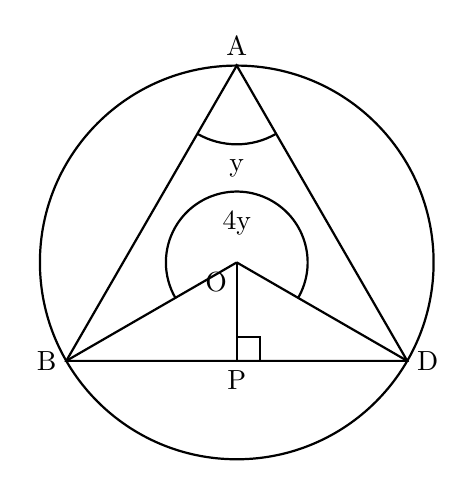
\begin{tikzpicture}[scale=1]

    % Define the center of the circle
    \coordinate (O) at (0,0);

    % Draw the circle
    \draw[thick] (O) circle (2.5);

    % Define the points on the circle
    \coordinate (A) at (90:2.5);
    \coordinate (B) at (210:2.5);
    \coordinate (D) at (330:2.5);

    % Define the point P on the chord BD
    \coordinate (P) at (0,-1.25);

    % Draw the triangle ABD
    \draw[thick] (A) -- (B) -- (D) -- cycle;

    % Draw the triangle OBD
    \draw[thick] (O) -- (B);
    \draw[thick] (O) -- (D);

    % Draw the perpendicular from O to BD
    \draw[thick] (O) -- (P);

    % Add the labels for the points
    \node[above] at (A) {A};
    \node[left] at (B) {B};
    \node[right] at (D) {D};
    \node[below] at (P) {P};
    \node[below left] at (O) {O};

    % Draw the angle arcs
    % Angle y centered at A (spanning from 240 degrees to 300 degrees)
    \draw[thick] (A) ++(240:1.0) arc (240:300:1.0);
    \node at (90:1.2) {y}; % Shifted down further

    % Angle 4y at O (drawn on top as a reflex angle)
    % Arc radius is slightly expanded so the label sits nicely underneath
    \draw[thick] (330:0.9) arc (-30:210:0.9);
    \node at (90:0.5) {4y}; % Shifted down further, closer to O

    % Draw the right angle symbol at P
    \draw[thick] (P) ++(0.3,0) -- ++(0,0.3) -- ++(-0.3,0);

\end{tikzpicture}